\documentclass[11pt]{article}
\usepackage[utf8]{inputenc}
\usepackage[T1]{fontenc}
\usepackage[left=1.5cm, right=1.5cm,top=1.5cm, bottom=1.5cm]{geometry}
\usepackage[colorlinks=true, allcolors=blue]{hyperref}
\usepackage{amsmath, amsfonts, lineno, graphicx, tikz}
\linenumbers


\begin{document}
\section{Discussion Nov 13th, 2025, Linz}

{\bf Evolution problem}: Let $\hat{\boldsymbol{y}} \in L^2(0, T; \mathbb{R}^N)$ a given target and $\gamma, \nu > 0$ two penalization parameters. We minimize the cost functional
\begin{equation}\label{eq:J}
\min_{\boldsymbol{y}, \boldsymbol{u}} J(\boldsymbol{y}, \boldsymbol{u}) := \frac12 \int_0^\top | \boldsymbol{y}(t) - \hat{\boldsymbol{y}}(t) |^2 \, dt +  \frac{\gamma}2 | \boldsymbol{y}(T) - \hat{\boldsymbol{y}}(T) |^2 + \frac{\nu}{2} \int_0^\top |\boldsymbol{u}(t)|^2 \, dt,
\end{equation}
such that
\begin{equation}\label{eq:heatdx}
\dot{\boldsymbol{y}}(t) + A \boldsymbol{y}(t) = \boldsymbol{u}(t), 
\quad
\boldsymbol{y}(0) = \boldsymbol{y}_0.
\end{equation}
Here, $\boldsymbol{y}(t), \hat{\boldsymbol{y}}(t), \boldsymbol{u}(t) \in \mathbb{R}^N$ are column vectors, $|\cdot|$ denotes the Euclidean norm, $A\in \mathbb{R}^{N\times N}$ can be seen as the discretization matrix of some spatial operators, and $\boldsymbol{y}_0 \in \mathbb{R}^N$ is a given initial vector. This problem can be seen as the semi-discretization in space of some linear PDE-constrained optimization problems. 


{\bf First-order optimality system}: The standard approach to treat this problem is to introduce a Lagrange multiplier $\boldsymbol{p} \in L^2(0, T; \mathbb{R}^N)$, and write the Lagrangian as
\[\mathcal{L}(\boldsymbol{y}, \boldsymbol{p}, \boldsymbol{u}) = J(\boldsymbol{y}, \boldsymbol{u}) - \int_0^\top \boldsymbol{p}^\top(t)\left(\dot{\boldsymbol{y}}(t) + A \boldsymbol{y}(t) - \boldsymbol{u}(t)\right)\, dt.\]
For any variation $\delta \boldsymbol{y} \in C^{\infty}(0, T; \mathbb{R}^N)$ with $\delta \boldsymbol{y}(0) = 0$, we have
\[\begin{aligned}
\partial_{\boldsymbol{y}}\mathcal{L}[\delta \boldsymbol{y}] = &\int_0^\top \left(\boldsymbol{y}(t) - \hat{\boldsymbol{y}}(t)\right)^\top\delta \boldsymbol{y}(t) \, dt + \gamma \left(\boldsymbol{y}(T) - \hat{\boldsymbol{y}}(T)\right)^\top\delta \boldsymbol{y}(T) \\
&+  \int_0^\top \boldsymbol{\dot p}^\top(t)\delta \boldsymbol{y}(t) \, dt - \int_0^\top (A^\top\boldsymbol{p})^\top(t) \delta \boldsymbol{y}(t) \, dt  - \boldsymbol{p}^\top(T)\delta \boldsymbol{y}(T) + \boldsymbol{p}^\top(0)\delta \boldsymbol{y}(0). 
\end{aligned}\]
Equating it to zero gives
\[-\dot{\boldsymbol{p}}(t) + A^\top \boldsymbol{p}(t) = \boldsymbol{y}(t) - \hat{\boldsymbol{y}}(t),
\quad
\boldsymbol{p}(T) = \gamma \left(\boldsymbol{y}(T) - \hat{\boldsymbol{y}}(T)\right).\]
Similarly, for any variation $\delta \boldsymbol{u} \in C^{\infty}(0, T; \mathbb{R}^N)$, we have
\[\partial_{\boldsymbol{u}}\mathcal{L}[\delta \boldsymbol{u}] = \int_0^\top \nu\boldsymbol{u}(t)^\top \delta \boldsymbol{u}(t) \, dt + \int_0^\top \boldsymbol{p}^\top(t)\delta \boldsymbol{u}(t) \, dt.\]
Equating it to zero gives
\[\boldsymbol{p}(t) + \nu \boldsymbol{u}(t) = 0.\]
We then obtain the optimality system
\begin{equation}\label{eq:optsys}
\begin{aligned}
\dot{\boldsymbol{y}}(t) + A \boldsymbol{y}(t) &= \boldsymbol{u}(t), && \boldsymbol{y}(0) = \boldsymbol{y}_0, \\
-\dot{\boldsymbol{p}}(t) + A^\top \boldsymbol{p}(t) &= \boldsymbol{y}(t) - \hat{\boldsymbol{y}}(t), &&\boldsymbol{p}(T) = \gamma \left(\boldsymbol{y}(T) - \hat{\boldsymbol{y}}(T)\right), \\
\nu \boldsymbol{u}(t) & = -\boldsymbol{p}(t),
\end{aligned}
\end{equation}
which can also be written in the integral form as
\[\begin{aligned}
\boldsymbol{y}(t) &= \boldsymbol{y}_0 + \int_0^\top \left( -A \boldsymbol{y}(t) + \boldsymbol{u}(t) \right)\, dt, \\
\boldsymbol{p}(t) &= \boldsymbol{p}(T) + \int_t^\top \left(-A^\top \boldsymbol{p}(t) + \boldsymbol{y}(t) - \hat{\boldsymbol{y}}(t) \right)\, dt, \\
\boldsymbol{u}(t) &= - \boldsymbol{p}(t) / \nu, \quad t\in(0, T).
\end{aligned}\]


{\bf Reduced cost functional}: To enter in the same optimization framework proposed in~\cite{CV2025}, we introduce the solution operator $\mathcal{S} : L^2(0, T; \mathbb{R}^N) \to L^2(0, T; \mathbb{R}^N)$ such that $\mathcal{S} \boldsymbol{u} = \boldsymbol{y}$. Substituting $\mathcal{S} \boldsymbol{u}$ into the cost functional gives 
\[J(\boldsymbol{u}) = J(\mathcal{S} \boldsymbol{u}, \boldsymbol{u}) = \frac12 \int_0^\top | \mathcal{S} \boldsymbol{u}(t) - \hat{\boldsymbol{y}}(t) |^2 \, dt +  \frac{\gamma}2 | \mathcal{S} \boldsymbol{u}(T) - \hat{\boldsymbol{y}}(T) |^2 + \frac{\nu}{2} \int_0^\top |\boldsymbol{u}(t)|^2 \, dt,\]
where we still use $J$ to denote the reduced cost functional. We can then write the optimization problem as $\min_{\boldsymbol{u}} J(\boldsymbol{u})$ and use the elimination approach proposed in~\cite{CV2025}. 


{\bf Decomposition}: There are two different ways to decompose the problem and write
\[J(\boldsymbol{u}_1, \boldsymbol{u}_2).\]
If we decompose the control variable $\boldsymbol{u}$ into two controls $\boldsymbol{u}_1(t)\in\mathbb{R}^{N_1}$ and $\boldsymbol{u}_2(t)\in\mathbb{R}^{N_2}$ with $N_1 + N_2 = N$. This is exactly in the spirit of~\cite{CV2025}, which corresponds to a space decomposition. In this case, the functional $J: L^2(0, T; \mathbb{R}^{N_1}) \times L^2(0, T; \mathbb{R}^{N_2}) \to \mathbb{R}$. Instead, one can also decompose the time interval $(0, T)$ into two subintervals $Q_1 := (T_0, T_1)$ and $Q_2 := (T_1, T_2)$ with $T_0 = 0$, $T_2 = T$ and $T_1\in(0, T)$. This corresponds to a time decomposition, and the two associated controls $\boldsymbol{u}_1(t)\in\mathbb{R}^{N}$, $t\in Q_1$ and $\boldsymbol{u}_2(t)\in\mathbb{R}^{N}$, $t\in Q_2$. In this case, the functional $J: L^2(T_0, T_1; \mathbb{R}^{N}) \times L^2(T_1, T_2; \mathbb{R}^{N}) \to \mathbb{R}$.
%LD: sorry for complexify the notation, may be convenient in case of having many subintervals.


As we are interested in the second case, let us derive the algorithm following the approach proposed in~\cite{CV2025}. Assuming that for every $\boldsymbol{u}_1$ the equation $\nabla_{\boldsymbol{u}_2}J(\boldsymbol{u}_1, \boldsymbol{u}_2) = 0$ admits a unique solution $\boldsymbol{u}_2$ and that  $\nabla_{\boldsymbol{u}_2\boldsymbol{u}_2}J(\boldsymbol{u}_1, \boldsymbol{u}_2)$ is invertible for every $(\boldsymbol{u}_1, \boldsymbol{u}_2)$, then applying the implicit function theorem, there exists a continuously differentiable mapping $h: L^2(T_0, T_1; \mathbb{R}^{N}) \to L^2(T_1, T_2; \mathbb{R}^{N})$ such that we can eliminate $\boldsymbol{u}_2$ and obtain $\nabla_{\boldsymbol{u}_2}J(\boldsymbol{u}_1, h(\boldsymbol{u}_1)) = 0$. We may apply the Newton iteration to solve the reduced optimality condition $F(\boldsymbol{u}_1) = \nabla_{\boldsymbol{u}_1}J(\boldsymbol{u}_1, h(\boldsymbol{u}_1)) = 0$. For iteration index $k = 0, 1, \ldots$, one solves
\[\boldsymbol{u}_1^{k+1} = \boldsymbol{u}_1^{k} - \left(JF(\boldsymbol{u}_1^{k})\right)^{-1}\nabla_{\boldsymbol{u}_1}J(\boldsymbol{u}_1^k, h(\boldsymbol{u}_1^k)),\]
which is exactly what has been shown in~\cite[Eq. 4]{CV2025}. 


As also discussed in~\cite{CV2025}, our ultimate goal is to solve the optimization problem. Thus, one can also perform such variable elimination on the objective function $J$, that is, $\tilde J(\boldsymbol{u}_1) := J(\boldsymbol{u}_1, h(\boldsymbol{u}_1))$, and then apply a gradient descent method to solve the minimization problem as  
\begin{equation}\label{eq:GradDesc}
\boldsymbol{u}_1^{k+1} = \boldsymbol{u}_1^{k} - \alpha \nabla \tilde J(\boldsymbol{u}_1^{k}).
\end{equation}
with $\alpha$ the step size satisfies $\tilde J(\boldsymbol{u}_1^k - \alpha \nabla \tilde J(\boldsymbol{u}_1^{k})) < \tilde J(\boldsymbol{u}_1^k)$. 


{\bf Algorithm}: The solving process can be resumed as:
\begin{enumerate}
\item For a given $\boldsymbol{u}_1^{k}$, one can find the state variable $\boldsymbol{y}_1^{k}$ with
\[\boldsymbol{y}_1^k(t) = \boldsymbol{y}_0 + \int_0^\top \left( -A \boldsymbol{y}_1^k(t) + \boldsymbol{u}_1^k(t) \right)\, dt.\]
This consists in applying the solution operator $\mathcal{S}_1 \boldsymbol{u}_1^{k}$.

\item Using the fact that $\boldsymbol{y}_2^{k}(T_1) = \boldsymbol{y}_1^{k}(T_1)$, one solves the system
\[\begin{aligned}
\boldsymbol{y}_2^{k}(t) &= \boldsymbol{y}_2^{k}(T_1) + \int_{T_1}^{t} \left( -A \boldsymbol{y}_2^{k}(t) + \boldsymbol{u}_2^{k}(t) \right)\, dt, \\
\boldsymbol{p}_2^{k}(t) &= \boldsymbol{p}_2^{k}(T_2) + \int_t^{T_2} \left(-A^\top \boldsymbol{p}_2^{k}(t) + \boldsymbol{y}_2^{k}(t) - \hat{\boldsymbol{y}}(t) \right)\, dt, \\
\boldsymbol{u}_2^{k}(t) &= - \boldsymbol{p}_2^{k}(t) / \nu, \quad t\in(T_1, T_2).
\end{aligned}\]
The above part consists in evaluating the mapping $\boldsymbol{u}_2^k = h(\boldsymbol{u}_1^{k})$. 

\item Update the control variable in $Q_1$ with
\[\boldsymbol{u}_1^{k+1} = \boldsymbol{u}_1^{k} - \alpha \left( \nabla_{\boldsymbol{u}_1} \tilde J\left(\boldsymbol{u}_1^{k}, h(\boldsymbol{u}_1^{k})\right) +  \nabla_{\boldsymbol{u}_2} \tilde J\left(\boldsymbol{u}_1^{k}, h(\boldsymbol{u}_1^{k})\right) h'(\boldsymbol{u}_1^{k})\right).\]
As the implicit mapping $h$ fulfils $\nabla_{\boldsymbol{u}_2}J(\boldsymbol{u}_1^{k}, h(\boldsymbol{u}_1^{k})) = 0$. The update can then be written as
\[\boldsymbol{u}_1^{k+1} = \boldsymbol{u}_1^{k} - \alpha  \nabla_{\boldsymbol{u}_1} \tilde J\left(\boldsymbol{u}_1^{k}, h(\boldsymbol{u}_1^{k})\right) = \boldsymbol{u}_1^{k} - \alpha (\boldsymbol{p}_1^k + \nu \boldsymbol{u}_1^k ),\]
where $\boldsymbol{p}_1^k$ is given by
\[\boldsymbol{p}_1^k(t) = \boldsymbol{p}_1^k(T_1) + \int_t^{T_1} \left(-A^\top \boldsymbol{p}_1^k(t) + \boldsymbol{y}_1^k(t) - \hat{\boldsymbol{y}}(t) \right)\, dt,\]
with $\boldsymbol{p}_1^k(T_1) = \boldsymbol{p}_2^k(T_1)$.
\end{enumerate}
Here, we are in the case with an exact solve of $\nabla_{\boldsymbol{u}_2}J(\boldsymbol{u}_1, \boldsymbol{u}_2) = 0$, as $\nabla_{\boldsymbol{u}_2}J(\boldsymbol{u}_1, \boldsymbol{u}_2) = \nu \boldsymbol{u}_2^{k} +\boldsymbol{p}_2^{k}$. 




\section{Discussion Dec 16th, 2025, Zoom}\label{sec:2}

We talked about the idea we had in Linz, and Gabriele mentioned his work with Parisa, which could be adapted to our case. Here is the idea (based on my understanding). 

{\bf Coarse-fine decomposition:} We consider two controls $ u_1 := (\boldsymbol u_{1f}, \boldsymbol u_{1c})^\top$ and $\boldsymbol u_2 := (\boldsymbol u_{2c}, \boldsymbol u_{2f})^\top$, where $\boldsymbol u_1$ is defined in the domain $Q_1 := Q_{1f} \cup Q_{1c}$, and $\boldsymbol u_2$ is defined in the domain $Q_2 := Q_{2c} \cup Q_{2f}$. Note that $Q_1 = Q_2 = Q = [0, T]$. Below is an illustration of these two decompositions.
\begin{center}
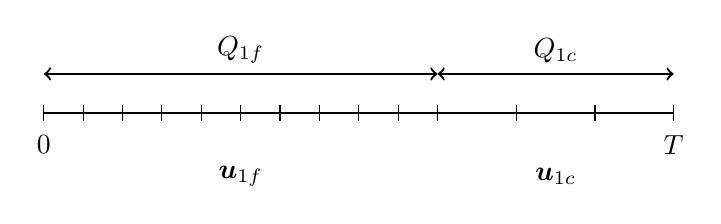
\begin{tikzpicture}
\draw [thick] (0, 0) -- (8, 0) ;
\foreach \x in {0, 0.5, 1, 1.5, 2, 2.5, 3, 3.5, 4, 4.5, 5, 6, 7, 8}{\draw (\x, 0.1) -- (\x, -0.1);}
\node at (0, -0.4) {0};
\node at (8, -0.4) {$T$};
\draw [thick, <->] (0, 0.5) -- (5, 0.5);
\node at (2.5, 0.8) {$Q_{1f}$};
\draw [thick, <->] (5, 0.5) -- (8, 0.5);
\node at (6.5, 0.8) {$Q_{1c}$};
\node at (2.5, -0.8) {$\boldsymbol u_{1f}$};
\node at (6.5, -0.8) {$\boldsymbol u_{1c}$};
\end{tikzpicture}
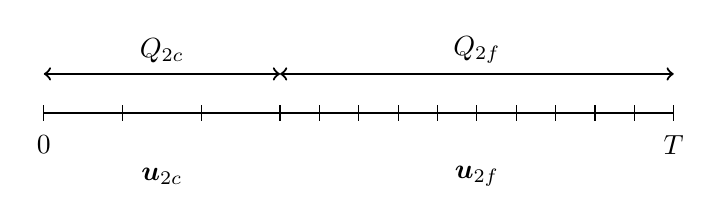
\begin{tikzpicture}
\draw [thick] (0, 0) -- (8, 0) ;
\foreach \x in {0, 1, 2, 3, 3.5, 4, 4.5, 5, 5.5, 6, 6.5, 7, 7.5, 8}{\draw (\x, 0.1) -- (\x, -0.1);}
\node at (0, -0.4) {0};
\node at (8, -0.4) {$T$};
\draw [thick, <->] (0, 0.5) -- (3, 0.5);
\node at (1.5, 0.8) {$Q_{2c}$};
\draw [thick, <->] (3, 0.5) -- (8, 0.5);
\node at (5.5, 0.8) {$Q_{2f}$};
\node at (1.5, -0.8) {$\boldsymbol u_{2c}$};
\node at (5.5, -0.8) {$\boldsymbol u_{2f}$};
\end{tikzpicture}
\end{center}
For each decomposition framework, we apply the gradient descent algorithm~\eqref{eq:GradDesc} to compute the optimal control $\boldsymbol u$, that is,
\begin{equation}\label{eq:GradDesc_u1u2}
\boldsymbol u_{1f}^{k+1} = \boldsymbol u_{1f}^k - \alpha \nabla_{\boldsymbol u_{1f}}J\left(\boldsymbol u_{1f}^{k+1}, h\left(\boldsymbol u_{1f}^{k+1}\right)\right),
\quad
\boldsymbol u_{2f}^{k+1} = \boldsymbol u_{2f}^k - \alpha \nabla_{\boldsymbol u_{2f}}J\left(h\left(\boldsymbol u_{2f}^{k+1}\right), \boldsymbol u_{2f}^{k+1}\right).
\end{equation}

Consider two restriction matrices $R_1$ and $R_2$ such that each part of $\boldsymbol u_j$ in the fine grid satisfies $\boldsymbol u_{1f}^k = R_1\boldsymbol u^k$ and $\boldsymbol u_{2f}^k = R_2\boldsymbol u^k$. Consider also two partition matrices $\tilde R_1$ and $\tilde R_2$ such that each new iteration is given by $\boldsymbol u^{k+1} = \tilde R_1^\top\boldsymbol u_{1f}^{k+1} + \tilde R_2^\top\boldsymbol u_{2f}^{k+1}$. Since there is an overlap between $Q_{1f}$ and $Q_{2f}$, we need these partition matrices to average $\boldsymbol u_{jf}^k$ on the overlap. The restriction matrices and partition matrices satisfy $\tilde R_1^\top R_1 + \tilde R_2^\top R_2 = I_N$. 

We define the matrix associated with the time discrete gradient $\nabla J$ by $H := \nu I_N + (A^\top)^{-1}A^{-1}$. In $Q_1$, the matrix $H^1 = H$ is written as
\[H^1 := \begin{bmatrix}
H_{ff}^1 & H_{fc}^1\\
H_{cf}^1 & H_{cc}^1
\end{bmatrix}.\]
Using the Schur complement, we can write the gradient descent of $\boldsymbol u_{1f}^k$ in~\eqref{eq:GradDesc_u1u2} as
\[\boldsymbol u_{1f}^{k+1} = \boldsymbol u_{1f}^k - \alpha \left(H_{ff}^1 - H_{fc}^1(H_{cc}^1)^{-1} H_{cf}^1\right)\boldsymbol u_{1f}^k.\]
Similarly, we have the matrix in $Q_2$ given by
\[H^2 := \begin{bmatrix}
H_{cc}^2 & H_{cf}^2\\
H_{fc}^2 & H_{ff}^2
\end{bmatrix},\]
and the gradient descent of $\boldsymbol u_{2f}^k$ in~\eqref{eq:GradDesc_u1u2} can be written as
\[\boldsymbol u_{2f}^{k+1} = \boldsymbol u_{2f}^k - \alpha \left(H_{ff}^2 - H_{fc}^2(H_{cc}^2)^{-1} H_{cf}^2\right)\boldsymbol u_{2f}^k.\]
Combining these two gradient descent parts gives the next update of $\boldsymbol u^k$ as
\[\boldsymbol u^{k+1} = \tilde R_1^\top\boldsymbol u_{1f}^{k+1} + \tilde R_2^\top\boldsymbol u_{2f}^{k+1} 
= \left[\tilde R_1^\top\left(I_1 - \alpha \left(H_{ff}^1 - H_{fc}^1(H_{cc}^1)^{-1} H_{cf}^1\right)\right)R_1 +  \tilde R_2^\top\left(I_2 - \alpha \left(H_{ff}^2 - H_{fc}^2(H_{cc}^2)^{-1} H_{cf}^2\right)\right)R_2 \right]\boldsymbol u^k.\]

We said to test this iterative matrix numerically with only fine grids everywhere to see its spectral radius. If the results are good, we can then talk about the next step. 


As I accidentally test first the elliptic case, which is in the MATLAB code {\tt EllipIterMatRho}, I also describe the elliptic problem briefly.


{\bf Elliptic problem:} Let $\hat y \in L^2(\Omega)$ be a given target and $\nu > 0$ a penalization parameter. We minimize the cost functional
\begin{equation}\label{eq:Jellip}
J(y, u) = \frac12\|y - \hat y\|^2_{L^2(\Omega)} + \frac{\nu}2\|u\|^2_{L^2(\Omega)}.
\end{equation}
such that 
\begin{equation}\label{eq:ellip}
- \Delta y = u \text{ in } \Omega,
\quad
y = 0 \text{ on } \partial\Omega.
\end{equation}
The Lagrangian is given by
\[\mathcal{L}(y, u, p) = \frac12\int_{\Omega}\left(y(x) - \hat y(x)\right)^2\,dx + \frac{\nu}2\int_{\Omega}\left(u(x)\right)^2\,dx - \int_{\Omega}\nabla p(x) \cdot \nabla y(x)\,dx + \int_{\Omega} p(x)u(x) \,dx.\]
The optimality system is given by
\begin{equation}\label{eq:OptSysEllip}
\begin{aligned}
- \Delta y &= u& \text{ in }& \Omega,& 
y &= 0& \text{ on }& \partial\Omega, \\
- \Delta p &= y - \hat y& \text{ in }& \Omega,&
p &= 0& \text{ on }& \partial\Omega, \\
\nu u + p &= 0& \text{ in }& \Omega.
\end{aligned}
\end{equation}




\section{Discussion Jan 20th, 2026, Zoom}
We mainly discussed the elliptic case and how to assemble the matrix without inverting globally the state matrix $A$ and the adjoint matrix $A^\top$ in $H$. Since the role of the matrices $H^1_{fc}$ and $H^1_{cf}$ in the MATLAB code {\tt EllipIterMatRho} or {\tt ParaIterMatRho} is unclear, we talked about analyzing the problem at the continuous level and seeing if we can invert "a partial fine partial coarse $-\Delta$" instead of "a full $-\Delta$". The idea is the following (based on my understanding). 


{\bf Continuous analysis:} We assume that there exist two operators $B_1: \Omega_1\to\Omega$ and $B_2: \Omega_2\to\Omega$ such that the elliptic optimal control problem~\eqref{eq:Jellip}-\eqref{eq:ellip} can be rewritten as: minimizing the cost functional
\[J(y_1, y_2, u) = \frac12\|y_1 + y_2 - \hat y\|^2_{L^2(\Omega)} + \frac{\nu}2\|u_1\|^2_{L^2(\Omega_1)} + \frac{\nu}2\|u_2\|^2_{L^2(\Omega_2)},\]
such that
\[- \Delta y_1 = B_1u_1 \text{ in } \Omega,
\quad
y_1 = 0 \text{ on } \partial\Omega,
\qquad
- \Delta y_2 = B_2u_2 \text{ in } \Omega,
\quad
y_2 = 0 \text{ on } \partial\Omega.\]
Here, we have $y_1 + y_2 = y$, but $u_1 + u_2\neq u$, instead $B_1u_1 + B_2u_2 = u$.

For a given $u_1$, we derive the optimality system associated with $u_2$,
\[\begin{aligned}
- \Delta y_2 &= B_2u_2& \text{ in }& \Omega,& 
y_2 &= 0& \text{ on }& \partial\Omega, \\
- \Delta p_2 &= y_1 + y_2 - \hat y& \text{ in }& \Omega,&
p_2 &= 0& \text{ on }& \partial\Omega, \\
\nu u_2+ B_2^\top p_2 &= 0& \text{ in }& \Omega,
\end{aligned}\]
where $B_2^\top: \Omega\to \Omega_2$. Applying a gradient descent to solve it, one gets 
\[u_2^{k+1} = u_2^k - \alpha \left(\nu u_2^k + B_2^\top \left((- \Delta)^{-2}B_2u_2^k + (- \Delta)^{-1}y_1^k- (- \Delta)^{-1}\hat y\right)\right).\]
Meanwhile, we derive the optimality system associated with $u_1$ for a given $u_2$,
\[\begin{aligned}
- \Delta y_1 &= B_1u_1& \text{ in }& \Omega,& 
y_1 &= 0& \text{ on }& \partial\Omega, \\
- \Delta p_1 &= y_1 + y_2- \hat y& \text{ in }& \Omega,&
p_1 &= 0& \text{ on }& \partial\Omega, \\
\nu u_1 + B_1^\top p_1 &= 0& \text{ in }& \Omega,
\end{aligned}\]
where $B_1^\top: \Omega\to \Omega_1$. Applying a gradient descent to solve it, one gets 
\[u_1^{k+1} = u_1^k - \alpha \left(\nu u_1^k + B_1^\top \left((- \Delta)^{-2}B_1u_1^k + (- \Delta)^{-1}y_2^k- (- \Delta)^{-1}\hat y\right)\right).\]
The next iteration $u^{k+1}$ is then defined by 
\[\begin{aligned}
u^{k+1} = &B_1u_1^{k+1} + B_2u_2^{k+1}\\
= &u^k - \alpha\nu u^k - \alpha(- \Delta)^{-2}u^k - \alpha (- \Delta)^{-1}y^k + 2\alpha (- \Delta)^{-1}\hat y\\
= &\left(1 - \alpha(\nu + (- \Delta)^{-2})\right)u^k + \alpha (- \Delta)^{-1}(2\hat y - y^k)
\end{aligned},\] 
where we need $B_1 B_1^\top = Id$ and $B_2 B_2^\top = Id$.


{\bf Question:} 1. What are $B_1$ and $B_2$ ? In particular, the cost functional is kind of saying that $\|u\|^2_{L^2(\Omega)} = \|B_1u_1+B_2u_2\|^2_{L^2(\Omega)} = \|u_1\|^2_{L^2(\Omega_1)} + \|u_2\|^2_{L^2(\Omega_2)}$.
2. I do not fully understand what "a partial fine partial coarse $-\Delta$" means at the continuous level. 


From my side, the role of the two operators $B_1, B_2$ is unclear to me, and we do not have any mesh (fine or coarse) at the continuous level. Therefore, I try to think if there are some alternatives. Our goal is to avoid solving a global $-\Delta$, and probably later use this coarse-fine decomposition idea in the discrete setting. Based on this, I have the following idea using classic domain decomposition.

{\bf Idea from DD:} We take the linear elliptic optimal control problem~\eqref{eq:Jellip}-\eqref{eq:ellip}, or more precesily the associated optimality system~\eqref{eq:OptSysEllip}. Consider two decompositions of the domain $(a, b)$: $\Omega_1 = (a, \beta_1) \cup (\alpha_1, b)$ and $\Omega_2 =  (a, \beta_2) \cup (\alpha_2, b)$, e.g see the illustration below. 
\begin{center}
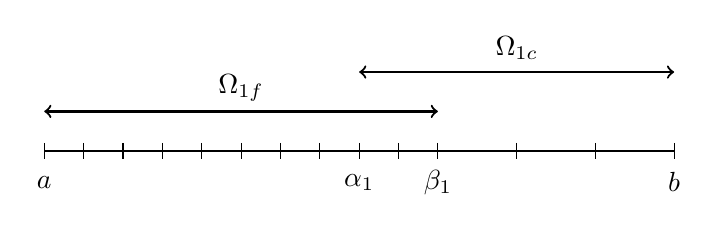
\begin{tikzpicture}
\draw [thick] (0, 0) -- (8, 0) ;
\foreach \x in {0, 0.5, 1, 1.5, 2, 2.5, 3, 3.5, 4, 4.5, 5, 6, 7, 8}{\draw (\x, 0.1) -- (\x, -0.1);}
\node at (0, -0.4) {$a$};
\node at (8, -0.4) {$b$};
\draw [thick, <->] (0, 0.5) -- (5, 0.5);
\node at (2.5, 0.8) {$\Omega_{1f}$};
\draw [thick, <->] (4, 1) -- (8, 1);
\node at (6, 1.3) {$\Omega_{1c}$};
\node at (5, -0.4) {$\beta_1$};
\node at (4, -0.4) {$\alpha_1$};
\end{tikzpicture}
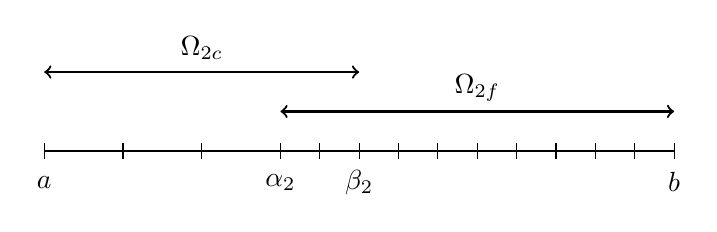
\begin{tikzpicture}
\draw [thick] (0, 0) -- (8, 0) ;
\foreach \x in {0, 1, 2, 3, 3.5, 4, 4.5, 5, 5.5, 6, 6.5, 7, 7.5, 8}{\draw (\x, 0.1) -- (\x, -0.1);}
\node at (0, -0.4) {$a$};
\node at (8, -0.4) {$b$};
\draw [thick, <->] (0, 1) -- (4, 1);
\node at (2, 1.3) {$\Omega_{2c}$};
\draw [thick, <->] (3, 0.5) -- (8, 0.5);
\node at (5.5, 0.8) {$\Omega_{2f}$};
\node at (4, -0.4) {$\beta_2$};
\node at (3, -0.4) {$\alpha_2$};
\end{tikzpicture}
\end{center}
They are very similar to the case that we talked about on Dec 16th, 2025. The only differences are that it is only in the space now, and there is an overlap in order to use the alternating Schwarz framework. Note that it is not necessary to have the overlap in the general decomposition setting.


For $\Omega_1$, we use the alternating Schwarz framework to decompose the optimality system~\eqref{eq:OptSysEllip}, which reads, 
\begin{equation}
\begin{aligned}
- \partial_{xx} y_{1f} &= u_{1f}& \text{ in }& (a, \beta_1),\\ 
y_{1f}(a) &= 0, \ y_{1f}(\beta_1) = y_{1c}(\beta_1),  \\
- \partial_{xx} p_{1f} &= y_{1f} - \hat y& \text{ in }& (a, \beta_1),\\
p_{1f}(a) &= 0, \ p_{1f}(\beta_1) = p_{1c}(\beta_1), \\
\nu u_{1f} + p_{1f} &= 0& \text{ in }& (a, \beta_1),
\end{aligned}
\qquad
\begin{aligned}
- \partial_{xx} y_{1c} &= u_{1c}& \text{ in }& (\alpha_1, b),\\ 
y_{1c}(b) &= 0, \ y_{1c}(\alpha_1) = y_{1f}(\alpha_1),  \\
- \partial_{xx} p_{1c} &= y_{1c} - \hat y& \text{ in }& (\alpha_1, b),\\
p_{1c}(b) &= 0, \ p_{1c}(\alpha_1) = p_{1f}(\alpha_1), \\
\nu u_{1c} + p_{1c} &= 0& \text{ in }& (\alpha_1, b),
\end{aligned}
\end{equation}
Similarly, we also apply such an alternating Schwarz framework in $\Omega_2$, which reads,
\begin{equation}
\begin{aligned}
- \partial_{xx} y_{2c} &= u_{2c}& \text{ in }& (a, \beta_2),\\ 
y_{2c}(a) &= 0, \ y_{2c}(\beta_2) = y_{2f}(\beta_2),  \\
- \partial_{xx} p_{2c} &= y_{2c} - \hat y& \text{ in }& (a, \beta_2),\\
p_{2c}(a) &= 0, \ p_{2c}(\beta_2) = p_{2f}(\beta_2), \\
\nu u_{2c} + p_{2c} &= 0& \text{ in }& (a, \beta_2),
\end{aligned}
\qquad
\begin{aligned}
- \partial_{xx} y_{2f} &= u_{2f}& \text{ in }& (\alpha_2, b),\\ 
y_{2f}(b) &= 0, \ y_{2f}(\alpha_2) = y_{2c}(\alpha_2),  \\
- \partial_{xx} p_{2f} &= y_{2f} - \hat y& \text{ in }& (\alpha_1, b),\\
p_{2f}(b) &= 0, \ p_{2f}(\alpha_2) = p_{2c}(\alpha_2), \\
\nu u_{2f} + p_{2f} &= 0& \text{ in }& (\alpha_2, b),
\end{aligned}
\end{equation}
Here, each $-\Delta$ (or each $-\partial_{xx}$) is only defined in each subdomain, and thus they are local. We now define our control variables by $u_1 := (u_{1f}, u_{1c})$ and $u_2 := (u_{2c}, u_{2f})$, we can then follow the same reasoning discussed in Section~\ref{sec:2} to analyze the behavior of the gradient descent iteration at the continuous level for the variable $u:=\tilde{\mathcal R}_1 u_{1f} + \tilde{\mathcal R}_2 u_{2f}$, where $\tilde{\mathcal R}_1, \tilde{\mathcal R}_2$ are the partition operators correspond to the partion matrices $\tilde R_1$ and $\tilde R_2$.


I do not know if this makes sense. Please let me know your opinion. 






\section{Discretization and numerical tests}
As I use two different approaches in the numerical tests, I briefly describe both approaches.

{\bf Discretize-then-optimize:} We describe here the discretize-then-optimize approach to solve the problem~\eqref{eq:J}-\eqref{eq:heatdx}. Let $0 = t_0 < t_1 < \ldots < t_M = T$ with uniform time step $\Delta t = T/M$. Denote $\boldsymbol{y}_m \approx \boldsymbol{y}(t_m)$, $\hat{\boldsymbol{y}}_m \approx \hat{\boldsymbol{y}}(t_m)$, $\boldsymbol{u}_m \approx \boldsymbol{u}(t_m)$ and $\boldsymbol{p}_m \approx \boldsymbol{p}(t_m)$. Applying the Crank-Nicolson time integration method for~\eqref{eq:heatdx} gives 
\begin{equation}\label{eq:heatdxCN}
\frac{\boldsymbol{y}_{m+1} - \boldsymbol{y}_{m}}{\Delta t} + A \frac{\boldsymbol{y}_{m+1} + \boldsymbol{y}_{m}}2 = \frac{\boldsymbol{u}_{m+1} + \boldsymbol{u}_{m}}2 
\ \Leftrightarrow \
\left(I_N + \frac{\Delta t}2 A\right) \boldsymbol{y}_{m+1} - \left(I_N - \frac{\Delta t}2 A\right) \boldsymbol{y}_{m} = \frac{\Delta t}2(\boldsymbol{u}_{m+1} + \boldsymbol{u}_{m}),
\end{equation}
for $m = 0, \ldots, M-1$ and a given $\boldsymbol{y}_0$. To keep consistence with the Crank-Nicolson method, we use the trapezodial rule for numerical integration of the cost function~\eqref{eq:J} and find
\begin{equation}\label{eq:JCN}
J_M(\boldsymbol{y}, \boldsymbol{u}) := \frac{\Delta t}4 \sum_{m=0}^{M-1} \left(|\boldsymbol{y}_{m+1} - \hat{\boldsymbol{y}}_{m+1}|^2 + |\boldsymbol{y}_m - \hat{\boldsymbol{y}}_m|^2\right)  +  \frac{\gamma}2 | \boldsymbol{y}_M - \hat{\boldsymbol{y}}_M |^2 + \frac{\nu\Delta t}4 \sum_{m=0}^{M-1} \left(|\boldsymbol{u}_{m+1}|^2 + |\boldsymbol{u}_m|^2\right).
\end{equation}
The discrete Lagrangian then reads
\begin{equation}\label{eq:LCN}
\mathcal{L} = J_M - \sum_{m=0}^{M-1} \boldsymbol{p}_{m+1}^\top\left(\left(I_N + \frac{\Delta t}2 A\right) \boldsymbol{y}_{m+1} - \left(I_N - \frac{\Delta t}2 A\right) \boldsymbol{y}_{m} - \frac{\Delta t}2(\boldsymbol{u}_{m+1} + \boldsymbol{u}_{m})\right).
\end{equation}
To obtain the discrete adjoint equation, one needs to do the "discrete integration by parts" in~\eqref{eq:LCN}, that is
\[\begin{aligned}
&\sum_{m=0}^{M-1} \boldsymbol{p}_{m+1}^\top\left(\left(I_N + \frac{\Delta t}2 A\right) \boldsymbol{y}_{m+1} - \left(I_N - \frac{\Delta t}2 A\right) \boldsymbol{y}_{m}\right) 
\\
= &\sum_{m=1}^{M} \boldsymbol{p}_{m}^\top\left(I_N + \frac{\Delta t}2 A\right) \boldsymbol{y}_{m} - \sum_{m=0}^{M-1} \boldsymbol{p}_{m+1}^\top\left(I_N - \frac{\Delta t}2 A\right) \boldsymbol{y}_{m}
\\
= &\sum_{m=1}^{M-1} \left(\left(I_N + \frac{\Delta t}2 A\right)^\top\boldsymbol{p}_{m} -  \left(I_N - \frac{\Delta t}2 A\right)^\top\boldsymbol{p}_{m+1}\right)^\top \boldsymbol{y}_{m} + \boldsymbol{p}_{M}^\top\left(I_N + \frac{\Delta t}2 A\right) \boldsymbol{y}_{M} - \boldsymbol{p}_{1}^\top\left(I_N - \frac{\Delta t}2 A\right) \boldsymbol{y}_{0}.
\end{aligned}\]
Meanwhile, we re-write the sum over $m$ of $\boldsymbol{y}_m$ in~\eqref{eq:JCN},
\[\frac{\Delta t}4 \sum_{m=0}^{M-1} |\boldsymbol{y}_{m+1} - \hat{\boldsymbol{y}}_{m+1}|^2 + \frac{\Delta t}4\sum_{m=0}^{M-1} |\boldsymbol{y}_m - \hat{\boldsymbol{y}}_m|^2 
= \frac{\Delta t}2\sum_{m=1}^{M-1} |\boldsymbol{y}_{m} - \hat{\boldsymbol{y}}_{m}|^2 + \frac{\Delta t}4|\boldsymbol{y}_{M} - \hat{\boldsymbol{y}}_{M}|^2 + \frac{\Delta t}4|\boldsymbol{y}_0 - \hat{\boldsymbol{y}}_0|^2.\]
We derive now the discrete adjoint equation 
\[\partial_{\boldsymbol{y}_m}\mathcal{L} = -\left(\left(I_N + \frac{\Delta t}2 A\right)^\top\boldsymbol{p}_{m} -  \left(I_N - \frac{\Delta t}2 A\right)^\top\boldsymbol{p}_{m+1}\right) +  \Delta t(\boldsymbol{y}_{m} - \hat{\boldsymbol{y}}_{m}),
\quad
m = 1,\ldots,M-1,\]
with the final condition
\[\partial_{\boldsymbol{y}_M}\mathcal{L} = -\left(I_N + \frac{\Delta t}2 A\right)^\top\boldsymbol{p}_M + \frac{\Delta t}2(\boldsymbol{y}_M - \hat{\boldsymbol{y}}_M) +  \gamma(\boldsymbol{y}_M - \hat{\boldsymbol{y}}_M).\]
We treat in a similar way of the sum related to $\boldsymbol{u}_m$ in~\eqref{eq:JCN}-\eqref{eq:LCN},
\[\begin{aligned}
\frac{\nu\Delta t}4 \sum_{m=0}^{M-1} |\boldsymbol{u}_{m+1}|^2 + \frac{\nu\Delta t}4 \sum_{m=0}^{M-1}|\boldsymbol{u}_m|^2 
&= \frac{\nu\Delta t}2 \sum_{m=1}^{M-1} |\boldsymbol{u}_{m}|^2 + \frac{\nu\Delta t}4 |\boldsymbol{u}_M|^2 + \frac{\nu\Delta t}4 |\boldsymbol{u}_0|^2,
\\
\frac{\Delta t}2\sum_{m=0}^{M-1} \boldsymbol{p}_{m+1}^\top\boldsymbol{u}_{m+1} + \frac{\Delta t}2\sum_{m=0}^{M-1} \boldsymbol{p}_{m+1}^\top\boldsymbol{u}_{m}
&= \frac{\Delta t}2\sum_{m=1}^{M-1} (\boldsymbol{p}_m^\top + \boldsymbol{p}_{m+1}^\top)\boldsymbol{u}_m + \frac{\Delta t}2\boldsymbol{p}_M^\top\boldsymbol{u}_M + \frac{\Delta t}2\boldsymbol{p}_1^\top\boldsymbol{u}_0.
\end{aligned}\]
This then gives the discrete optimality condition
\[\partial_{\boldsymbol{u}_m}\mathcal{L} = \frac{\Delta t}2(\boldsymbol{p}_m + \boldsymbol{p}_{m+1}) + \nu\Delta t \boldsymbol{u}_{m},
\quad 
m = 1,\ldots, M-1,
\quad
\partial_{\boldsymbol{u}_M}\mathcal{L} = \frac{\nu\Delta t}2 \boldsymbol{u}_M + \frac{\Delta t}2\boldsymbol{p}_M,
\quad
\partial_{\boldsymbol{u}_0}\mathcal{L} = \frac{\nu\Delta t}2 \boldsymbol{u}_0 + \frac{\Delta t}2\boldsymbol{p}_1.\]
Equating these partial derivatives to zero gives the discrete optimality system using the Crank-Nicolson method,
\begin{equation}\label{eq:optsysCNDto}
\begin{aligned}
\left(I_N + \frac{\Delta t}2 A\right) \boldsymbol{y}_{m+1} - \left(I_N - \frac{\Delta t}2 A\right) \boldsymbol{y}_{m} &= \frac{\Delta t}2(\boldsymbol{u}_{m+1} + \boldsymbol{u}_{m}),&
m &= 0,\ldots, M-1,
\\
\left(I_N + \frac{\Delta t}2 A^\top\right)\boldsymbol{p}_m -  \left(I_N - \frac{\Delta t}2 A^\top\right)\boldsymbol{p}_{m+1} &=  \Delta t(\boldsymbol{y}_{m} - \hat{\boldsymbol{y}}_{m}),&
m &= 1,\ldots, M-1,
\\
\left(I_N + \frac{\Delta t}2 A^\top\right)\boldsymbol{p}_M &= \left(\frac{\Delta t}2 + \gamma\right)(\boldsymbol{y}_M - \hat{\boldsymbol{y}}_M),
\\
\nu \boldsymbol{u}_{m} &= -\frac{\boldsymbol{p}_m + \boldsymbol{p}_{m+1}}2,&
m &= 1,\ldots, M-1,
\\
\nu\boldsymbol{u}_M &= -\boldsymbol{p}_M,
\quad \nu \boldsymbol{u}_0 = -\boldsymbol{p}_1.
\end{aligned}
\end{equation}
Denote by $\boldsymbol X_1 := (\boldsymbol{y}_1, \ldots, \boldsymbol{y}_M)^\top$, $\boldsymbol X_2 := (\boldsymbol{p}_1, \ldots, \boldsymbol{p}_M)^\top$ and $\boldsymbol X_3 := (\boldsymbol{u}_0, \ldots, \boldsymbol{u}_M)^\top$. Note that there is no $\boldsymbol{p}_0$ in the discretize-then-optimize approach, since the discrete adjoint state starts from $\boldsymbol{p}_1$ associated with the first CN discrete state equation. Note also that the size of $\boldsymbol X_3$ is different from the others. The all-at-once block matrix form is given by
\[\tilde A \boldsymbol X = \boldsymbol F,
\quad
\tilde A = \begin{bmatrix}
\tilde A_{11} & \boldsymbol0 & \tilde A_{13}\\
\tilde A_{21} & \tilde A_{22} & \boldsymbol0\\
\boldsymbol0 & \tilde A_{32} & \tilde A_{33}
\end{bmatrix},
\quad 
\boldsymbol X = \begin{bmatrix}
\boldsymbol X_1\\
\boldsymbol X_2\\
\boldsymbol X_3
\end{bmatrix},
\quad
\boldsymbol F = \begin{bmatrix}
\boldsymbol F_1 \\
\boldsymbol F_2 \\
\boldsymbol0
\end{bmatrix}.\]
Each block matrix $\tilde A_{ij}$ is given by
\[\begin{aligned}
\tilde A_{11} &= \begin{bmatrix}
I_N + \frac{\Delta t}2 A & \\
-\left(I_N - \frac{\Delta t}2 A\right) & I_N + \frac{\Delta t}2 A \\
&\ddots &\ddots\\
& &-\left(I_N - \frac{\Delta t}2 A\right) & I_N + \frac{\Delta t}2 A\\
& & &-\left(I_N - \frac{\Delta t}2 A\right) & I_N + \frac{\Delta t}2 A
\end{bmatrix},
\\
\tilde A_{13} &= \begin{bmatrix}
-\frac{\Delta t}2I_N & -\frac{\Delta t}2I_N &\\
&\ddots &\ddots\\
& &-\frac{\Delta t}2I_N & -\frac{\Delta t}2I_N
\end{bmatrix},
\quad
\tilde A_{21} = \begin{bmatrix}
-\Delta tI_N & \\
& -\Delta tI_N \\
& &\ddots\\
& & &-\Delta tI_N \\
& & & & -\left(\frac{\Delta t}2+\gamma\right)I_N
\end{bmatrix},
\\
\tilde A_{22} &= \begin{bmatrix}
I_N + \frac{\Delta t}2 A^\top & -\left(I_N - \frac{\Delta t}2 A^\top\right)\\
&I_N + \frac{\Delta t}2 A^\top & -\left(I_N - \frac{\Delta t}2 A^\top\right)\\
& &\ddots &\ddots\\
& & &I_N + \frac{\Delta t}2 A^\top & -\left(I_N - \frac{\Delta t}2 A^\top\right)\\
& & & &I_N + \frac{\Delta t}2 A^\top
\end{bmatrix},
\\
\tilde A_{32} &= \begin{bmatrix}
I_N\\
\frac12 I_N & \frac12 I_N \\
&\ddots &\ddots\\
& &\frac12 I_N & \frac12 I_N\\
& & &I_N
\end{bmatrix},
\quad
\tilde A_{33} = \begin{bmatrix}
\nu I_N \\
&\ddots\\
& &\nu I_N
\end{bmatrix}.
\end{aligned}\]
Note that $\tilde A_{13}\in\mathbb{R}^{NM\times N(M+1)}$ and $\tilde A_{32}\in\mathbb{R}^{N(M+1)\times NM}$ are two rectangular matrices. Note also that $\tilde A_{22} = \tilde A_{11}^\top\in\mathbb{R}^{NM\times NM}$. The right-hand side vector is given by
\[\boldsymbol{F}_1 = \begin{bmatrix}
\left(I_N - \frac{\Delta t}2 A\right)\boldsymbol{y}_0\\
0\\
\vdots\\
0
\end{bmatrix},
\quad
\boldsymbol{F}_2 = \begin{bmatrix}
-\Delta t\hat{\boldsymbol{y}}_1\\
\vdots\\
-\Delta t\hat{\boldsymbol{y}}_{M-1}\\
-\left(\frac{\Delta t}2+\gamma\right)\hat{\boldsymbol{y}}_M
\end{bmatrix}.\]
Bring everything to the control variable, in this case $\boldsymbol X_3$, gives
\[(\tilde A_{33} + \tilde A_{32}\tilde A_{22}^{-1}\tilde A_{21} \tilde A_{11}^{-1}\tilde A_{13})\boldsymbol X_3 + \tilde A_{32}\tilde A_{22}^{-1}\boldsymbol F_2 - \tilde A_{32}\tilde A_{22}^{-1}\tilde A_{21}\tilde A_{11}^{-1}\boldsymbol F_1 = 0.\]
Therefore, the matrix $H$ appeared in the Discussion Dec 16th, 2025 (Section~\ref{sec:2}) should be $H:=\tilde A_{33} + \tilde A_{32}\tilde A_{22}^{-1}\tilde A_{21} \tilde A_{11}^{-1}\tilde A_{13}$ using the discretize-then-optimize approach.

\medskip 

{\bf Reduced system:} We can substitute $\boldsymbol{u}_m$ by $\boldsymbol{p}_m$ to obtain the discrete reduced optimality system
\begin{equation}\label{eq:optsysCNDto-reduced}
\begin{aligned}
\left(I_N + \frac{\Delta t}2 A\right) \boldsymbol{y}_{m+1} - \left(I_N - \frac{\Delta t}2 A\right) \boldsymbol{y}_{m} +\frac{\Delta t}{4\nu}(\boldsymbol{p}_m + 2\boldsymbol{p}_{m+1} + \boldsymbol{p}_{m+2}) &= 0,&
m &= 1,\ldots, M-2,
\\
\left(I_N + \frac{\Delta t}2 A\right) \boldsymbol{y}_1 - \left(I_N - \frac{\Delta t}2 A\right) \boldsymbol{y}_0 +\frac{\Delta t}{4\nu}(3\boldsymbol{p}_1 + \boldsymbol{p}_2) &= 0,
\\
\left(I_N + \frac{\Delta t}2 A\right) \boldsymbol{y}_M - \left(I_N - \frac{\Delta t}2 A\right) \boldsymbol{y}_{M-1} +\frac{\Delta t}{4\nu}(3\boldsymbol{p}_M + \boldsymbol{p}_{M-1})&=0,
\\
\left(I_N + \frac{\Delta t}2 A^\top\right)\boldsymbol{p}_m -  \left(I_N - \frac{\Delta t}2 A^\top\right)\boldsymbol{p}_{m+1} - \Delta t\boldsymbol{y}_{m}&= -\Delta t\hat{\boldsymbol{y}}_{m},&
m &= 1,\ldots, M-1,
\\
\left(I_N + \frac{\Delta t}2 A^\top\right)\boldsymbol{p}_M - \left(\frac{\Delta t}2 + \gamma\right)\boldsymbol{y}_M &= -\left(\frac{\Delta t}2 + \gamma\right)\hat{\boldsymbol{y}}_M.
\end{aligned}
\end{equation}
The block matrix form of the reduced system is given by
\[\tilde A \boldsymbol{X} = \boldsymbol{F},
\quad
\tilde A = \begin{bmatrix}
\tilde A_{11} & \tilde A_{12}\\
\tilde A_{21} & \tilde A_{22}
\end{bmatrix},
\quad
\boldsymbol{X} = \begin{bmatrix}
\boldsymbol{X}_1 \\
\boldsymbol{X}_2
\end{bmatrix},
\quad
\boldsymbol{F} = \begin{bmatrix}
\boldsymbol{F}_1 \\
\boldsymbol{F}_2
\end{bmatrix},\]
with
\[\tilde A_{12} = \begin{bmatrix}
\frac{3\Delta t}{4\nu}I_N & \frac{\Delta t}{4\nu}I_N\\
\frac{\Delta t}{4\nu}I_N & \frac{\Delta t}{2\nu}I_N &\frac{\Delta t}{4\nu}I_N \\
&\ddots &\ddots&\ddots\\
& &\frac{\Delta t}{4\nu}I_N & \frac{\Delta t}{2\nu}I_N &\frac{\Delta t}{4\nu}I_N \\
& & &\frac{\Delta t}{4\nu}I_N & \frac{3\Delta t}{4\nu}I_N
\end{bmatrix}.\]
The rest matrices are the same as in the full all-at-once matrix form. This reduced form is used in the MATLAB code {\tt DtovsOtd}, where these block matrices are constructed by the function {\tt BuildCNMatrixDto}, and the right-hand side vector is constructed by the function {\tt BuildCNRhsDto}. This serves as the implemented solver for the discretize-then-optimize approach.


\medskip

{\bf Optimize-then-discretize}: Note that the discrete optimality system obtained in~\eqref{eq:optsysCNDto} is different from applying directly the Crank-Nicolson method to discretize the optimality system~\eqref{eq:optsys}. For comparison, we also show the optimize-then-discretize approach to solve the problem~\eqref{eq:J}-\eqref{eq:heatdx}, which consists of discretizing directly the optimality system~\eqref{eq:optsys} using the Crank-Nicolson method.
\begin{equation}\label{eq:optsysCNOtd}
\begin{aligned}
\frac{\boldsymbol{y}_{m+1} - \boldsymbol{y}_{m}}{\Delta t} + \frac A2 (\boldsymbol{y}_{m+1} + \boldsymbol{y}_{m})&= \frac12(\boldsymbol{u}_{m+1} + \boldsymbol{u}_{m}),&
m &= 0,\ldots, M-1,\\
-\frac{\boldsymbol{p}_{m+1} - \boldsymbol{p}_{m}}{\Delta t} + \frac{A^\top}2 (\boldsymbol{p}_{m+1} + \boldsymbol{p}_{m})&=  \frac12(\boldsymbol{y}_{m+1} - \hat{\boldsymbol{y}}_{m+1} + \boldsymbol{y}_{m} - \hat{\boldsymbol{y}}_{m}),&
m &= 0,\ldots, M-1, \\
\boldsymbol{p}_M &= \gamma(\boldsymbol{y}_{M} - \hat{\boldsymbol{y}}_{M}),& \\
\nu\boldsymbol{u}_M &= -\boldsymbol{p}_M,&
m &= 0,\ldots, M. 
\end{aligned}
\end{equation}
As in the discretize-then-optimize approach, we denote by $\boldsymbol X_1 := (\boldsymbol{y}_0, \ldots, \boldsymbol{y}_M)^\top$, $\boldsymbol X_2 := (\boldsymbol{p}_0, \ldots, \boldsymbol{p}_M)^\top$ and $\boldsymbol X_3 := (\boldsymbol{u}_0, \ldots, \boldsymbol{u}_M)^\top$. Note that all $\boldsymbol X_j$ here have the same size, as we discretize the adjoint equation directly, and we have the $\boldsymbol p_0$ term. Using the same notations as in the previous approach, the all-at-once block matrix form is given by
\[\tilde A \boldsymbol X = \boldsymbol F,
\quad
\tilde A = \begin{bmatrix}
\tilde A_{11} & \boldsymbol0 & \tilde A_{13}\\
\tilde A_{21} & \tilde A_{22} & \boldsymbol0\\
\boldsymbol0 & \tilde A_{32} & \tilde A_{33}
\end{bmatrix},
\quad 
\boldsymbol X = \begin{bmatrix}
\boldsymbol X_1\\
\boldsymbol X_2\\
\boldsymbol X_3
\end{bmatrix},
\quad
\boldsymbol F = \begin{bmatrix}
\boldsymbol F_1 \\
\boldsymbol F_2 \\
\boldsymbol0
\end{bmatrix}.\]
Each block matrix $\tilde A_{ij} \in \mathbb{R}^{N(M+1)\times N(M+1)}$ is given by
\[\begin{aligned}
\tilde A_{11} &= \begin{bmatrix}
I_N & \\
-\left(I_N - \frac{\Delta t}2 A\right) & I_N + \frac{\Delta t}2 A \\
&\ddots &\ddots\\
& &-\left(I_N - \frac{\Delta t}2 A\right) & I_N + \frac{\Delta t}2 A\\
& & &-\left(I_N - \frac{\Delta t}2 A\right) & I_N + \frac{\Delta t}2 A
\end{bmatrix},
\\
\tilde A_{13} &= \begin{bmatrix}
0  \\
-\frac{\Delta t}{2}I_N & -\frac{\Delta t}{2}I_N & \\
&\ddots &\ddots&\\
& &-\frac{\Delta t}{2}I_N &- \frac{\Delta t}{2}I_N
\end{bmatrix},
\quad
\tilde A_{21} = \begin{bmatrix}
-\frac{\Delta t}{2}I_N & -\frac{\Delta t}{2}I_N  \\
& -\frac{\Delta t}{2}I_N & -\frac{\Delta t}{2}I_N  \\
& &\ddots&\ddots\\
& & &-\frac{\Delta t}{2}I_N & -\frac{\Delta t}{2}I_N  \\
& & & & -\gamma I_N
\end{bmatrix},
\\
\tilde A_{22} &= \begin{bmatrix}
I_N + \frac{\Delta t}2 A^\top & -\left(I_N - \frac{\Delta t}2 A^\top\right)\\
&I_N + \frac{\Delta t}2 A^\top & -\left(I_N - \frac{\Delta t}2 A^\top\right)\\
& &\ddots &\ddots\\
& & &I_N + \frac{\Delta t}2 A^\top & -\left(I_N - \frac{\Delta t}2 A^\top\right)\\
& & & &I_N 
\end{bmatrix},
\\
\tilde A_{32} &= \begin{bmatrix}
I_N\\
&\ddots\\
& &I_N
\end{bmatrix},
\quad
\tilde A_{33} = \begin{bmatrix}
\nu I_N \\
&\ddots\\
& &\nu I_N
\end{bmatrix}.
\end{aligned}\]
The right-hand side vector is given by
\[\boldsymbol{F}_1 = \begin{bmatrix}
\boldsymbol{y}_0\\
0\\
\vdots\\
0
\end{bmatrix},
\quad
\boldsymbol{F}_2 = \begin{bmatrix}
-\frac{\Delta t}2(\hat{\boldsymbol{y}}_0 + \hat{\boldsymbol{y}}_1)\\
\vdots\\
-\frac{\Delta t}2(\hat{\boldsymbol{y}}_{M-1} + \hat{\boldsymbol{y}}_M)\\
-\gamma\hat{\boldsymbol{y}}_M
\end{bmatrix}.\]
Bring everything to the control variable $\boldsymbol X_3$ gives
\[(\tilde A_{33} + \tilde A_{22}^{-1}\tilde A_{21} \tilde A_{11}^{-1}\tilde A_{13})\boldsymbol X_3 + \tilde A_{22}^{-1}\boldsymbol F_2 - \tilde A_{22}^{-1}\tilde A_{21}\tilde A_{11}^{-1}\boldsymbol F_1 = 0.\]
Therefore, the matrix $H$ appeared in the discussion on Dec 16th, 2025 (Section~\ref{sec:2}) should be $H:=\tilde A_{33} + \tilde A_{22}^{-1}\tilde A_{21} \tilde A_{11}^{-1}\tilde A_{13}$ using the optimize-then-discretize approach.

\medskip 

{\bf Reduced system:} We can substitute $\boldsymbol{u}_m$ by $\boldsymbol{p}_m$ to obtain 
\begin{equation}\label{eq:optsysCNOtd-reduced}
\begin{aligned}
\left(I_N + \frac{\Delta t}2 A\right) \boldsymbol{y}_{m+1} - \left(I_N - \frac{\Delta t}2 A\right) \boldsymbol{y}_{m} +\frac{\Delta t}{2\nu}(\boldsymbol{p}_m + \boldsymbol{p}_{m+1}) &= 0,&
m &= 0,\ldots, M-1,
\\
\left(I_N + \frac{\Delta t}2 A^\top\right)\boldsymbol{p}_m -\left(I_N - \frac{\Delta t}2 A^\top\right)\boldsymbol{p}_{m+1}  -\frac{\Delta t}2(\boldsymbol{y}_{m+1} + \boldsymbol{y}_{m})&=  -\frac{\Delta t}2(\hat{\boldsymbol{y}}_{m+1} + \hat{\boldsymbol{y}}_{m}),&
m &= 0,\ldots, M-1,
\\
\boldsymbol{p}_M - \gamma\boldsymbol{y}_M &= -\gamma \hat{\boldsymbol{y}}_M.
\end{aligned}
\end{equation}
The block matrix form of the reduced system is given by
\[\tilde A \boldsymbol{X} = \boldsymbol{F},
\quad
\tilde A = \begin{bmatrix}
\tilde A_{11} & \tilde A_{12}\\
\tilde A_{21} & \tilde A_{22}
\end{bmatrix},
\quad
\boldsymbol{X} = \begin{bmatrix}
\boldsymbol{X}_1 \\
\boldsymbol{X}_2
\end{bmatrix},
\quad
\boldsymbol{F} = \begin{bmatrix}
\boldsymbol{F}_1 \\
\boldsymbol{F}_2
\end{bmatrix},\]
with 
\[\tilde A_{12} = \begin{bmatrix}
0 & \\
\frac{\Delta t}{2\nu}I_N & \frac{\Delta t}{2\nu}I_N & \\
&\ddots &\ddots&\\
& &\frac{\Delta t}{2\nu}I_N & \frac{\Delta t}{2\nu}I_N & \\
& & &\frac{\Delta t}{2\nu}I_N & \frac{\Delta t}{2\nu}I_N
\end{bmatrix}.\]
The rest matrices are the same as in the full all-at-once matrix form. This reduced form is used in the MATLAB code {\tt DtovsOtd}, where these block matrices are constructed by the function {\tt BuildCNMatrixOtd}, and the right-hand side vector is constructed by the function {\tt BuildCNRhsOtd}. This serves as the implemented solver for the optimize-then-discretize approach.

\medskip

{\bf Description of MATLAB code {\tt DtovsOtd}:} To test these two approaches, we use the following manufactured solutions, 
\[y(x, t) = \sin(\pi x)(2t^2 + t), 
\quad 
\hat y(x, t) = \nu\sin(\pi x)((\pi^4+1/\nu)(2t^2 + t) - 4), 
\quad 
p(x, t) = -\nu\sin(\pi x)(\pi^2(2t^2 + t) + 4t + 1),\]
and a special penalization parameter $\gamma$ to ensure the final condition,
\[\gamma = \frac{\pi^2(2T^2+T) + 4T + 1}{\pi^4(2T^2+T) - 4},\]
for $x\in (0, 1)$. These solutions satisfy the 1D reduced optimality system
\[\begin{aligned}
\partial_t y - \partial_{xx} y &= -\nu^{-1} p,& 
y(0, t) &= y(1, t) = 0, &
y(x, 0) &=0, 
\\
-\partial_t p - \partial_{xx} p &= y - \hat y,& 
p(0, t) &= p(1, t) = 0, &
p(x, T) &= \gamma(y(x, T) - \hat y(x, T)).
\end{aligned}\]
We set $T=1$, $\nu=1$ and $h_t=h_x=\{2^{-3}, \ldots, 2^{-8}\}$.
\begin{center}
\includegraphics[scale = 0.2]{Dto_T1_L1_al1_Err.png}
\includegraphics[scale = 0.2]{Otd_T1_L1_al1_Err.png}
\end{center}
On the left is the error decay when refining the mesh for the discretize-then-optimize approach~\eqref{eq:optsysCNDto-reduced}, and on the right is the case for the optimize-then-discretize approach~\eqref{eq:optsysCNOtd-reduced}. It is second-order for the optimize-then-discretize approach, as we use CN scheme to discretize the forward-backward system. However, it is only first-order for the adjoint variable in the discretize-then-optimize approach.


{\bf Description of MATLAB code {\tt EllipIterMatRho}:}
Consider a one dimensional domain $\Omega = (a, b)$, we discretize $-\Delta$ by the centered finite difference that leads to a symmetric tri-diagonal matrix $A\in\mathbb{R}^{N\times N}$. The discrete all-at-one system then reads
\begin{equation}\label{eq:OptSysEllipFD}
\begin{bmatrix}
A & 0 & -I_N\\
-I_N & A^\top & 0\\
0 & I_N & \nu I_N
\end{bmatrix}
\begin{bmatrix}
\boldsymbol y\\
\boldsymbol p\\
\boldsymbol u
\end{bmatrix}
= 
\begin{bmatrix}
0\\
-\hat{\boldsymbol y}\\
0
\end{bmatrix},
\end{equation}
or equivalently $H\boldsymbol u = A^\top\hat{\boldsymbol y}$ with $H:=\nu I_N + (AA^\top)^{-1}$.


I follow the idea proposed in Section~\ref{sec:2}, except that I tested for the above linear elliptic optimal control problem. We consider two decompositions of the domain $\Omega$: $\Omega_1 = \Omega_{11} \cup \Omega_{12}$ and $\Omega_2 =  \Omega_{21} \cup \Omega_{22}$ with $\Omega_1 = \Omega_2 = \Omega$.
\begin{center}
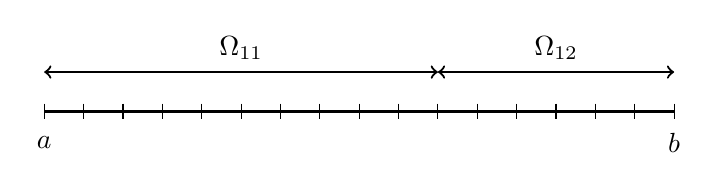
\begin{tikzpicture}
\draw [thick] (0, 0) -- (8, 0) ;
\foreach \x in {0, 0.5, 1, 1.5, 2, 2.5, 3, 3.5, 4, 4.5, 5, 5.5, 6, 6.5, 7, 7.5, 8}{\draw (\x, 0.1) -- (\x, -0.1);}
\node at (0, -0.4) {$a$};
\node at (8, -0.4) {$b$};
\draw [thick, <->] (0, 0.5) -- (5, 0.5);
\node at (2.5, 0.8) {$\Omega_{11}$};
\draw [thick, <->] (5, 0.5) -- (8, 0.5);
\node at (6.5, 0.8) {$\Omega_{12}$};
\end{tikzpicture}
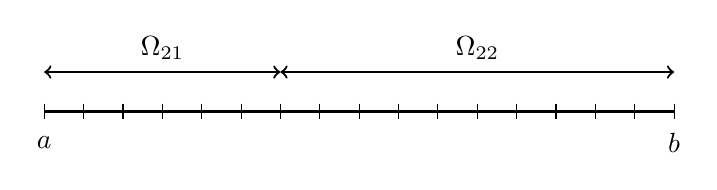
\begin{tikzpicture}
\draw [thick] (0, 0) -- (8, 0) ;
\foreach \x in {0, 0.5, 1, 1.5, 2, 2.5, 3, 3.5, 4, 4.5, 5, 5.5, 6, 6.5, 7, 7.5, 8}{\draw (\x, 0.1) -- (\x, -0.1);}
\node at (0, -0.4) {$a$};
\node at (8, -0.4) {$b$};
\draw [thick, <->] (0, 0.5) -- (3, 0.5);
\node at (1.5, 0.8) {$\Omega_{21}$};
\draw [thick, <->] (3, 0.5) -- (8, 0.5);
\node at (5.5, 0.8) {$\Omega_{22}$};
\end{tikzpicture}
\end{center}
In each domain $\Omega_j$, $j = 1, 2$, we solve the same optimality system~\eqref{eq:OptSysEllipFD} using a different decomposition. This corresponds to two control vectors $\boldsymbol u_1 := (\boldsymbol u_{11}, \boldsymbol u_{12})^\top$ and $\boldsymbol u_2 := (\boldsymbol u_{21}, \boldsymbol u_{22})^\top$, each satisfies a linear system $H^j \boldsymbol u_j = A^\top\hat{\boldsymbol y}$ associated with the problem defined in $\Omega_j$, $j = 1, 2$. Based on the structure of $\Omega_j$, the two matrices satisfy $H^1 = H^2 = H$ and are given by  
\[H^1 = \begin{bmatrix}
H^1_{11} & H^1_{12} \\
H^1_{21} & H^1_{22}
\end{bmatrix},
\quad
H^2 = \begin{bmatrix}
H^2_{11} & H^2_{12} \\
H^2_{21} & H^2_{22}
\end{bmatrix},\]
where each block is a truncation of the matrix $H$. The Schur complement $S_1$ defined by $S_1 := H^1_{11} - H^1_{12}(H^1_{22})^{-1}H^1_{21}$ is used to solve for $\boldsymbol u_{11}$, and the Schur complement $S_1$ defined by $S_2 := H^2_{22} - H^2_{21}(H^2_{11})^{-1}H^2_{12}$ is used to solve for $\boldsymbol u_{22}$. We apply the gradient descent algorithm to solve both $\boldsymbol u_{11}$ and $\boldsymbol u_{22}$ iteratively as explained in Section~\ref{sec:2}, and compute the spectral radius of the iterative matrix $\tilde R_1^\top (I - \alpha_1 S_1) R_1  + \tilde R_2^\top (I - \alpha_2 S_2)  R_2$.



{\bf Description of MATLAB code {\tt ParaIterMatRho}:} This part tries to test the idea given in the discussion on Dec 16th, 2025 (Section~\ref{sec:2}) using only a fine mesh everywhere. The matrix $H$ associated with the gradient is different depending on the two approaches. In the discretize-then-optimize approach, $H:=\tilde A_{33} + \tilde A_{32}\tilde A_{22}^{-1}\tilde A_{21} \tilde A_{11}^{-1}\tilde A_{13}$; in the optimize-then-discretize approach, $H:=\tilde A_{33} + \tilde A_{22}^{-1}\tilde A_{21} \tilde A_{11}^{-1}\tilde A_{13}$. Details are given above for each approach. Apart from that, the rest follows the same steps as in the elliptic case, and we compute the spectral radius of the associated iterative matrix $\tilde R_1^\top (I - \alpha_1 S_1) R_1  + \tilde R_2^\top (I - \alpha_2 S_2)  R_2$.

\bibliography{biblio}
\bibliographystyle{siam}
\end{document}